% Generated by system/tools/paper_figures.py from experiments/e2-*/scores.csv; do not edit.
\definecolor{usulan}{HTML}{2A78D6}
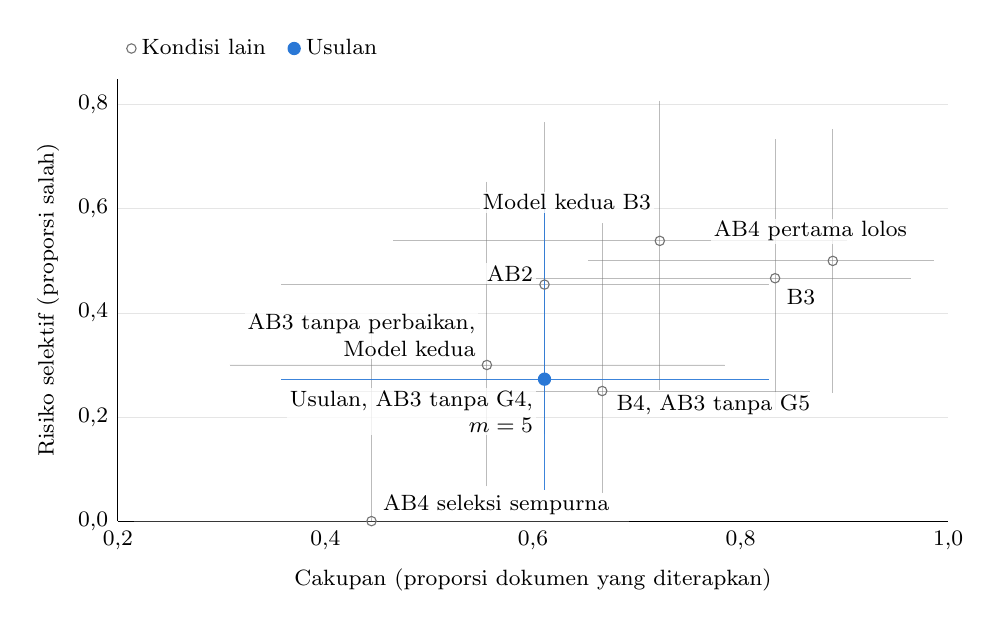
\begin{tikzpicture}
\begin{axis}[width=\columnwidth, height=7.2cm, scale only axis=false, xmin=0.2, xmax=1, ymin=0, ymax=0.85,
  xlabel={Cakupan (proporsi dokumen yang diterapkan)},
  ylabel={Risiko selektif (proporsi salah)},
  label style={font=\footnotesize}, tick label style={font=\footnotesize},
  xtick={0.2,0.4,0.6,0.8,1}, ytick={0,0.2,0.4,0.6,0.8},
  xticklabel style={/pgf/number format/.cd, fixed, fixed zerofill, precision=1, use comma},
  yticklabel style={/pgf/number format/.cd, fixed, fixed zerofill, precision=1, use comma},
  ymajorgrids, grid style={gray!20, line width=0.3pt}, axis lines*=left, tick style={draw=none},
  legend style={font=\footnotesize, draw=none, fill=none, at={(0,1.02)}, anchor=south west,
    legend columns=2, /tikz/every even column/.append style={column sep=6pt}}]
\addplot[only marks, mark=o, mark size=1.7pt, draw=black!55, fill=black!55,
  error bars/.cd, x dir=both, x explicit, y dir=both, y explicit,
  error bar style={draw=black!55, line width=0.35pt, opacity=0.45}, error mark=none]
  coordinates {(0.8333,0.4667) += (0.1309,0.2675) -= (0.2475,0.2540)
    (0.6667,0.2500) += (0.1999,0.3219) -= (0.2567,0.1951)
    (0.6111,0.4545) += (0.2159,0.3117) -= (0.2537,0.2871)
    (0.5556,0.3000) += (0.2291,0.3525) -= (0.2480,0.2333)
    (0.8889,0.5000) += (0.0974,0.2535) -= (0.2360,0.2535)
    (0.4444,0.0000) += (0.2480,0.3694) -= (0.2291,0.0000)
    (0.7222,0.5385) += (0.1808,0.2693) -= (0.2570,0.2871)};
\addlegendentry{Kondisi lain}
\addplot[only marks, mark=*, mark size=2.2pt, draw=usulan, fill=usulan,
  error bars/.cd, x dir=both, x explicit, y dir=both, y explicit,
  error bar style={draw=usulan, line width=0.35pt, opacity=0.9}, error mark=none]
  coordinates {(0.6111,0.2727) += (0.2159,0.3370) -= (0.2537,0.2125)};
\addlegendentry{Usulan}
\node[font=\footnotesize, anchor=north east, inner sep=1pt, fill=white, fill opacity=0.8, text opacity=1, xshift=-3pt, yshift=-3pt, align=right] at (axis cs:0.6111,0.2727) {Usulan, AB3 tanpa G4,\\$m = 5$};
\node[font=\footnotesize, anchor=north west, inner sep=1pt, fill=white, fill opacity=0.8, text opacity=1, xshift=3pt, yshift=-3pt, align=right] at (axis cs:0.8333,0.4667) {B3};
\node[font=\footnotesize, anchor=west, inner sep=1pt, fill=white, fill opacity=0.8, text opacity=1, xshift=4pt, yshift=-5pt, align=right] at (axis cs:0.6667,0.2500) {B4, AB3 tanpa G5};
\node[font=\footnotesize, anchor=east, inner sep=1pt, fill=white, fill opacity=0.8, text opacity=1, xshift=-3pt, yshift=4pt, align=right] at (axis cs:0.6111,0.4545) {AB2};
\node[font=\footnotesize, anchor=south east, inner sep=1pt, fill=white, fill opacity=0.8, text opacity=1, xshift=-3pt, yshift=2pt, align=right] at (axis cs:0.5556,0.3000) {AB3 tanpa perbaikan,\\Model kedua};
\node[font=\footnotesize, anchor=south east, inner sep=1pt, fill=white, fill opacity=0.8, text opacity=1, xshift=28pt, yshift=6pt, align=right] at (axis cs:0.8889,0.5000) {AB4 pertama lolos};
\node[font=\footnotesize, anchor=south west, inner sep=1pt, fill=white, fill opacity=0.8, text opacity=1, xshift=3pt, yshift=1pt, align=right] at (axis cs:0.4444,0.0000) {AB4 seleksi sempurna};
\node[font=\footnotesize, anchor=south east, inner sep=1pt, fill=white, fill opacity=0.8, text opacity=1, xshift=-2pt, yshift=10pt, align=right] at (axis cs:0.7222,0.5385) {Model kedua B3};
\end{axis}
\end{tikzpicture}
